% !TEX encoding = UTF-8 Unicode
\documentclass[a4paper]{article}

\usepackage[utf8]{inputenc}
\usepackage{erk}
\usepackage{times}
\usepackage{graphicx}
\usepackage{cite}
\usepackage{array}
\usepackage[top=22.5mm, bottom=22.5mm, left=22.5mm, right=22.5mm]{geometry}

\usepackage[english]{babel}

% local definitions
\def\footnotemark{}%  to avoid footnote on cover page

\begin{document}
%make title
\title{New dataset of emotional and color responses to music}

\author{Primož Godec$^{1}$, Matevž Pesek$^{1}$, Mojca Poredoš$^{1}$, Gregor Strle$^{2}$,\\ Jože Guna$^{3}$, Emilija Stojmenova$^{3}$, Matevž Pogačnik$^{3}$ and Matija Marolt$^{1}$} % use ^1, ^2 for author(s) from different institutions

\affiliation{$^{1}$University of Ljubljana, Faculty of computer and information science \\ 
$^{2}$Institute of Ethnomusicology, Scientfic Research Centre of the Slovenian Academy of Sciences and Arts \\
$^{3}$University of Ljubljana, Faculty of Electrotechnics}

\email{E-mail: \{matevz.pesek, matija.marolt\}@fri.uni-lj.si, \{primoz.godec, mojca.poredos\}@lgm.fri.uni-lj.si \\ gregor.strle@zrc-sazu.si,  \{joze.guna, emilija.stojmenova, matevz.pogacnik\}@fe.uni-lj.si}

\maketitle

\begin{abstract}{Abstract}
This paper presents a new dataset gathered containing perceived and induced emotions for 200 audio clips. The gathered dataset also provides users' association of color for each clip, along with users' demographic and personal data, such as users' emotion state, preferred genres, music experience and daily inference, and others. With an online survey we collected more than 7000 responses for a dataset of 200 audio excerpts, thus providing about 37 user responses per clip. We introduced a new methodology for gathering user perception of emotions in a form of two new interfaces - the MoodGraph and MoodStripe. We present a preliminary evaluation of classifying the present emotions with a regression algorithm on the gathered dataset, and perform a comparison towards other datasets and algorithms.
\end{abstract}

\section{Introduction}

The intention of this study is to provide a dataset for the research in a highly subjective field of multi-modal perception and the connecting relations between the music, colors and emotions. The problem has been previously well formalised in the field of psychology; however, it is our intention to tackle the problem in the domain of signal processing. In order to achieve the desired goal, we gathered a dataset possibly covering several aspects such as personal information, current mood state of the user and his music taste and experience. Many researchers have worked on similar problems; however, there are several undiscovered relations that brought the problem to our attention. 

Music mood estimation has become a recognised task in the past year; the music information retrieval evaluation exchange (MIREX) organises mood classification task since 2007. 

Several machine-learning-driven approaches have already been presented for the mood estimation task. Schmi\-dt et al. \cite{schmidt2009projection} use regression for mood classification. Panda et al. \cite{panda2013multi} use support vector machines, k-nearest neighbours, C4.5 and naive bayes. Support vector machine was also used by \cite{laurier2007audio}. Barthet et al. \cite{barthet2013design} use support vector regression for classification. 

There are several applications of the mood estimation, for example in order to boost the efficiency of music recommendation systems. In order to develop such music recommendation system, an annotated dataset is needed. Several datasets were gathered. We present a brief overview of the publicly available datasets. Eerola et al \cite{eerola2010comparison} performed a gathering of the film music dataset. Each sound track provides a single mean rating with label and values in three-dimensional valence-arousal-tension model. The dataset contains values for 361 film music clips. The Mood Swings Turk Dataset contains on average 17 valence-arousal ratings for each of the 240 audio clips \cite{schmidt2011modeling}. Clips in this dataset are mostly excerpts from popular music. The Cal500 provides mood labels for 500 western popular songs \cite{turnbull2008semantic} encompassing 3 annotations per song. The MTV Music Dataset contains 5 bipolar valence-arousal ratings for 192 popular songs \cite{schuller2010mister}. These songs were obtained from the MTV channel playlists.

In order to obtain a statistically significant amount of user responses per song, we performed user response gathering over a dataset for 200 audio clips. In addition to responses on music clips, we collected some other participants' demographic data and perception of mood. This data might help us to understand difference in responses to audio clips and possibly find correlations between users with similar background. In order to evaluate the usefulness of the collected data and possibly highlight the importance of the relations between the modalities and the user's personal data, we performed a preliminary evaluation of the mood estimation algorithm using the regression for valence-arousal prediction, as described in \cite{schmidt2009projection}. This algorithm was tested on our dataset and Mood Swing Turk dataset \cite{schmidt2011modeling}.

The paper is structured as follows: section 2 describes the survey and it design, section 3 provides analyses of the gathered data and survey evaluation and section 4 concludes the paper and describes our future work.


\section{Online survey}

For the user responses gathering procedure, an online survey was used. In order to fully anticipate possible drawbacks of previously collected annotations, we carefully picked the set of labels for emotions by performing a preliminary study over a large label set and identifying the key labels most fitting the majority of participants.

Some basic emotion labels exist, e.g. \cite{dalgleish1999handbook}; however, there is no standard set in music and mood research to our knowledge. Others choose label sets intuitively, without any explanations \cite{wu2013spectral}. In order to use an optimal set of labels, we prepared preliminary survey.

Participants were asked describe their emotional state on scale from 1 to 7 for each of 48 emotional labels. We also observed responses about color perception on a continuous color wheel used to describe connection between mood and colors. Depending on results of this questionnaire we selected 17 basic emotion labels which strongly correlate to three basic components that explain 64\% of the variance to the dataset. Depending on user responses and results we also decided to restrict continuous color wheel; we developed a discete-scale color wheel containing 49 colors. 

\subsection{The survey}

By incorporating the conclusions of the preliminary survey, we performed a second  online survey on a larger scale of participants. We structured the survey into three sections. We captured user personal background and demographic in first part. Users were asked to answer the demographic questions about the following aspects: age, area of living and native language along with information about users' music education, genre preference, and the amount of time listening to the music. We speculate about the importance of such data being gathered along with the mood perception responses for the annotated dataset. 

Second part contains questions about user perceptions of mood and connection between color and mood. First we asked for user current mood state with three different tasks. User had place his current mood in valence-arousal space. The valence-arousal space is a 2D plane to describe pleasantness and activeness of the mood. We also inquired about the user's perception of current mood by selecting best-matching color in a color wheel. We introduced a new interface, described in \cite{pesek2014gathering}, named the MoodStripe (Figure \ref{moodstripe}). The user was asked to drag each label describing the emotion onto a one-dimensional canvas. The canvas possesses a continuous scale between \textit{completely absent} and \textit{significantly expressed}.

The second part contained also two tasks that directly capture music mood perception. First, the user was asked to place 10 basic emotional labels onto valence-arousal space according to perception of emotion. We developed a second interface named \textit{the  MoodGraph} (see Fig. \ref{moodgraph}), extending the moodStripe into a two dimensional canvas. The user was also asked to pick a best-matching color for each music excerpt.

\begin{figure}[ht]
\centering
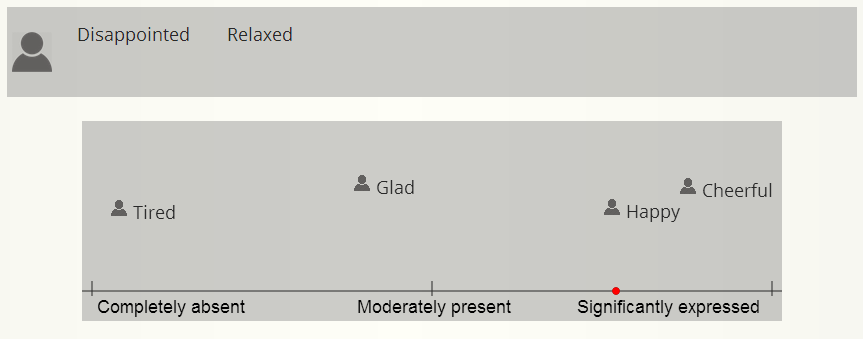
\includegraphics[width=80mm]{moodstripe.png}
\caption{The new interface used in our survey, named \textit{the MoodStripe}. With the drag-and-drop technique, a user can place emotion labels onto the plane depending on how the dragged emotion expressed. Placing the label towards the left side of the canvas reflects the absence of the emotions, where as placing it towards the right expresses the presence.}
\label{moodstripe}
\end{figure}

\begin{figure}[ht]
\centering
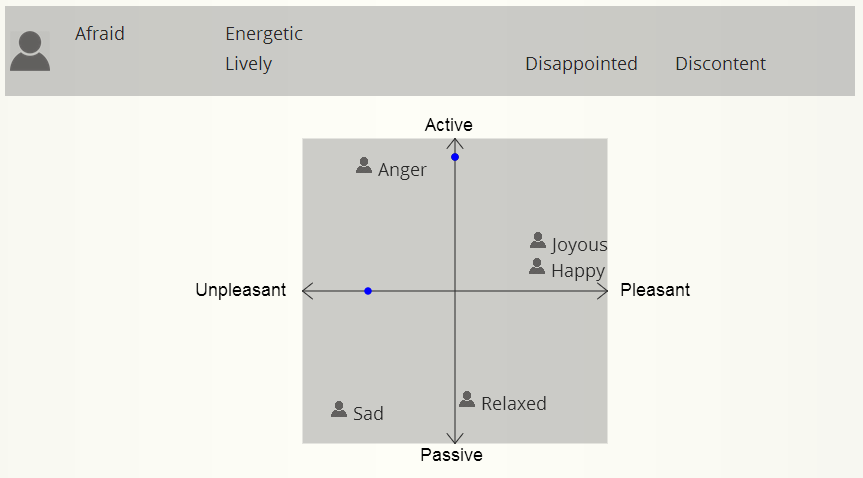
\includegraphics[width=80mm]{moodgraph.png}
\caption{The MoodGraph - a two-dimensional extension of the moodStripe interface, with two categories. Each positioned label is marked with an icon representing the category.}
\label{moodgraph}
\end{figure}

In the last part of our survey the user was asked to make two actions for each of 10 audio clips. Clips are 15 second long and was randomly selected from base of 200 clips. All selected audio clips are for most of users unknown, to avoid bias because of familiarity of song. We gathered music from four sources. Eighty songs was chosen from the free online music service Jamendo. We selected songs from as many genre as possible. Next 80 clips was from film music dataset and is described here \cite{eerola2010comparison}. We also provide 20 clips from collection of slovenian folk music collection and 20 of the contemporary electro-acoustic music collection. 

%The second part contained also two tasks that directly capture music mood perception. First, the user was asked to place emotional labels matching the emotions of a music excerpt onto valence-arousal space. The labels were split into two categories - the \textit{perceived } and the \textit{induced} emotions. We developed a second interface named \textit{the MoodGraph} (see Fig. \ref{moodgraph}), extending the moodStripe into a two dimensional canvas with two categories. The user was also asked to pick a best-matching color for each music excerpt.

For each clip we asked user to select color, that he think best describes music clip. User was also asked select emotion labels that best describe clip and place them in valence-arousal space. We provide two group of labels. The user was selecting between 10 labels for induced and between 14 labels for perceived and place it in valence-arousal space using MoodGraph (Figure \ref{moodgraph}). 

\section{Results}

\begin{table*}[t]
\caption{Results in prediction valence arousal using regression}
\begin{tabular}{| l | c | c | c | c | c | c |}
\hline
Feature & Avg. distance & Near. distance & Avg. dist in sdt & Avg. distance & Near. distance & Avg. dist in sdt \\
\hline
MFCC & 0.2060 & 0.0595 & 0.4870 & 0.2448 & 0.0641 & 0.6514\\
Chroma & 0.2215 & 0.0614 & 0.4993 & 0.3316 & 0.1026 & 0.8940\\
\hline
\end{tabular}
\label{regressionresults}
\end{table*}

We collected 7187 responses from 1357 participants in our survey. The dataset contains 200 audio clips, resulting in collecting 37 responses per audio clip on average. To our knowledge, there is no mood-music dataset with such high ratio per clip. Each response contains at least two positioned labels - one describing a perceived and one an induced emotion, and a picked color tone for the audio clip. 

The following section presents a preliminary demographic analysis, along with a performed experiment using the regression for mood estimation on the collected dataset.

\subsection{Demographic analysis}

The basic demographic characteristics of the 952 partici-
pants are as follows. The average age of participants was
26.5 years, the youngest had 15, the oldest 64 years. 65\%
of participants are women, 66\% are from urban areas.
50\% have no music education, 47\% do not play instru-
ments or sing. The amount of music listening per day is
evenly spread from less than 1 hour to over 4 hours. 3\%
claimed they were under the influence of drugs when tak-
ing the survey.

\subsection{Predicting valence-arousal values using regression}

[PRIŠEL DO TUKAJ]

We performed a simple mood estimation using the regression on the collected dataset. We implemented the regression algorithm used in \cite{schmidt2009projection}.Least squares method on MFCC \cite{logan2000mel} and Chroma \cite{bello2005robust} features was used. MFCCs was calculated with the cepstral coefficients 20, Chroma was calculated using 12 bins. Features was calculated using LibROSA python library on a 15 seconds audio clips from dataset. Dataset was divided into 2 parts. First set contains 70\% of dataset and was used for training algorithm using least squares \cite{abdi2007method}. Training was made with mean values of valence and arousal. This algorithm returns mapping vector $b$ as result. Second set (containing other 30\% of dataset) was used to test valence and arousal prediction. Values was calculated separately for valence and arousal using following equation: $$y = X b$$ where $X$ is feature matrix. Each row represents one vector of features for audio clip. $b$ is vector calculated with regression algorithm and maps values from feature space to valence or arousal value. $y$ is vector of predictions for valence or arousal. 

\begin{figure}[ht]
\centering
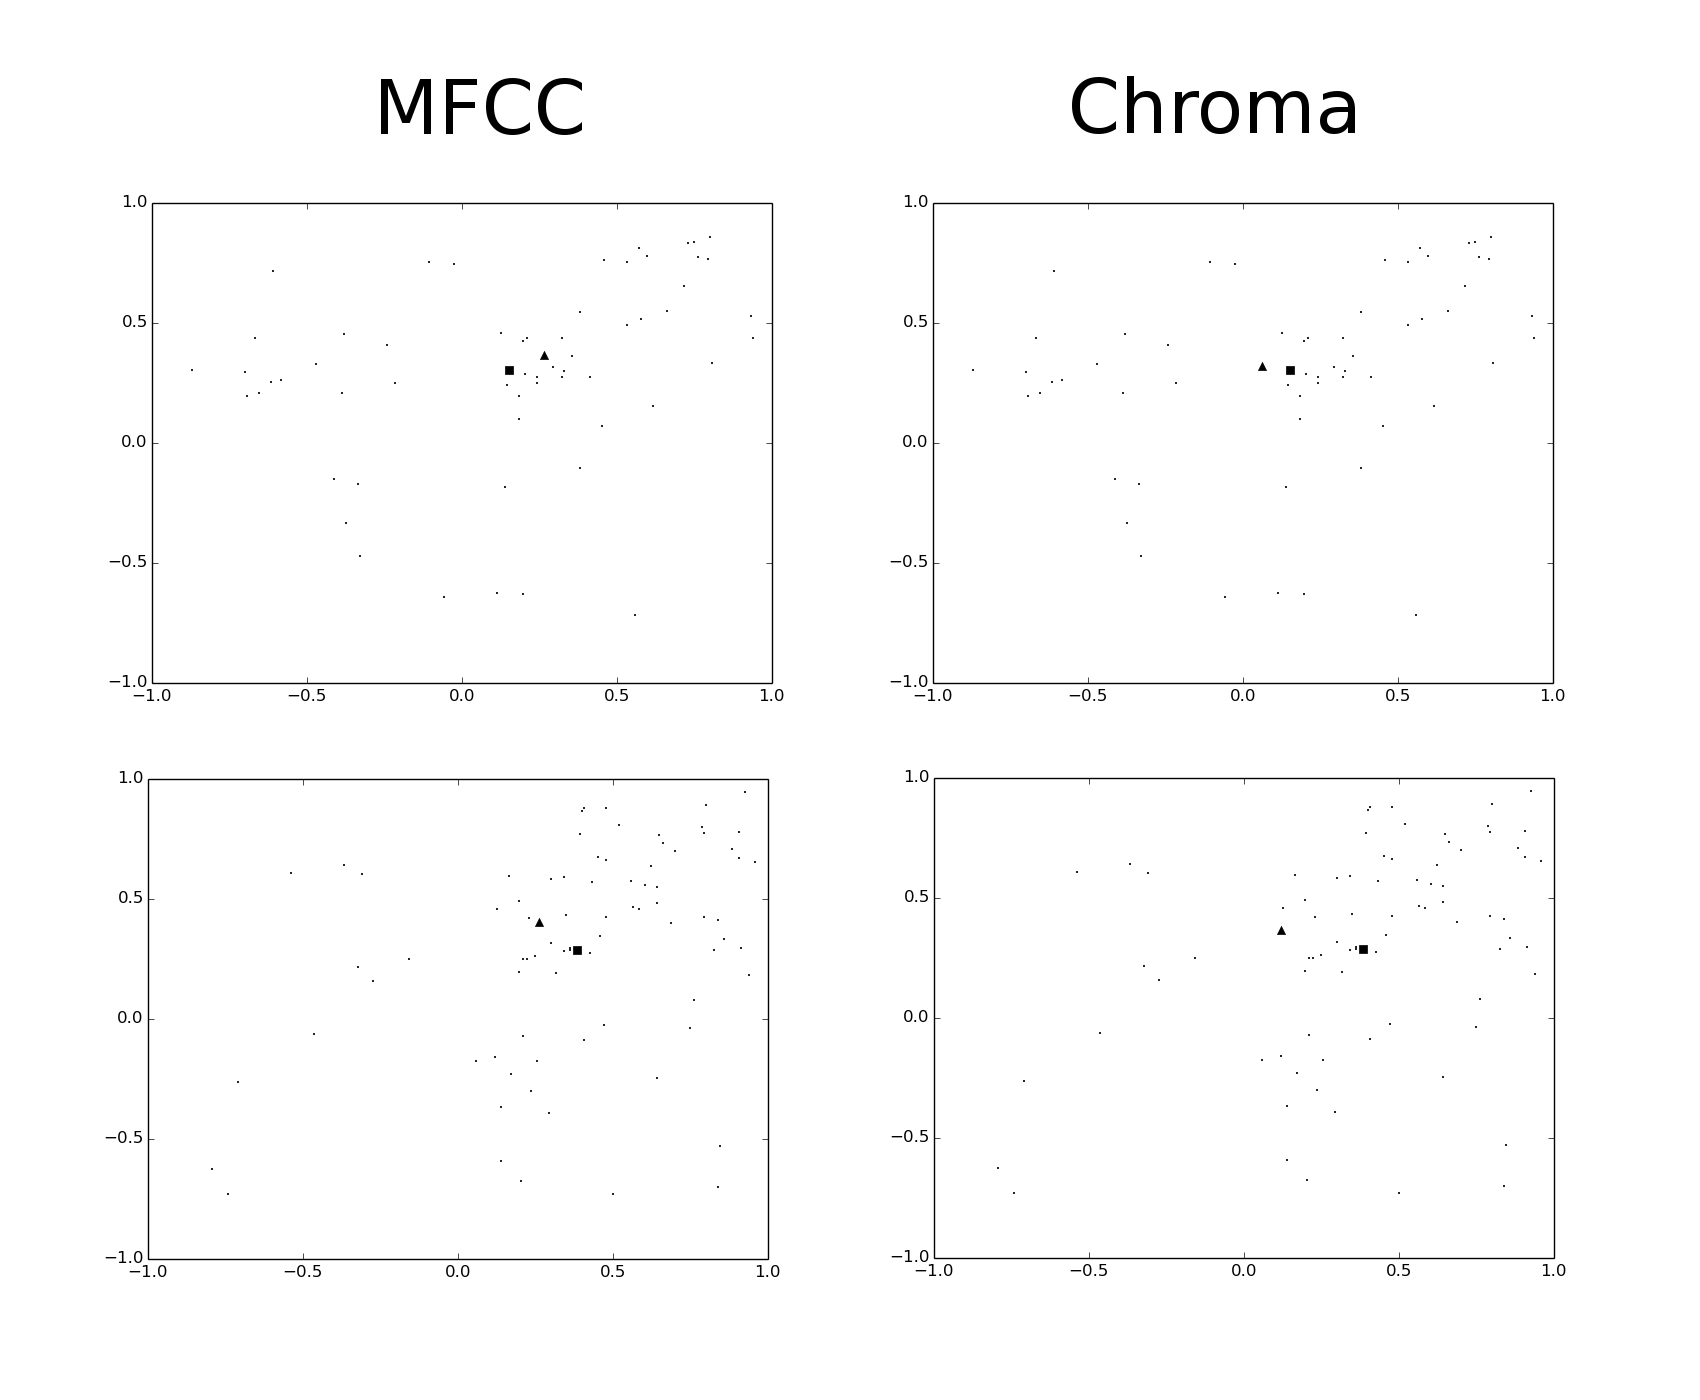
\includegraphics[width=80mm]{graphs.png}
\caption{Image shows 4 valence-arousal spaces, where pleasantness raises from left to right on x axis and activeness for bottom to top on z axis. The first row shows prediction on songs with id 413 using MFCC and Chroma. Same is shown for song 571 in the second row. The triangle shows regression algorithm prediction, the square shows mean value of all valence-arousal values gathered with survey. Dots show all valence-arousal values gathered.  }
\label{graphs}
\end{figure}

Results using regression algorithm are shown in table \ref{regressionresults}. For regression with MFCC and regression with Chroma average distance between estimated and mean valence-arousal value was calculated. We also provide the average distance to nearest value in dataset and the average distance between the mean valence-arousal point and the prediction, measured in the size of the standard deviation of data. Same algorithm was also used on the features Schmidt et al. provides for Mood Swing dataset \cite{schmidt2011modeling} to compare results. 

Our results shows that there is better correlation between MFCC and valence-arousal than this between Chro\-ma and valence arousal. From table is also seen that we got better result on our dataset than results on Mood Swing dataset are.  

We also performed regression algorithm on chroma features calculated with Compositional hierarchical model described in \cite{pesek2013chord}, what gave us the best results on regression algorithm. Average distance is 0.1862, distance to nearest value is 0.0719 and distance measured in standard deviation is 0.4459. 

\newcolumntype{L}[1]{>{\raggedright\arraybackslash}p{#1}}
\newcolumntype{C}[1]{>{\centering\arraybackslash}p{#1}}
\newcolumntype{R}[1]{>{\raggedleft\arraybackslash}p{#1}}

\begin{table}[h]
\caption{Average distances between the predictions and the mean valence-arousal value separately for valence and arousal}
\begin{tabular}{|L{1.2cm}|C{1.7cm}|C{1.7cm}| C{1.8cm}|}
\hline
 & MFCC & Chroma & MP Chroma \\
\hline
Valence & 0.1734 & 0.1826 & 0.1494\\
Arousal & 0.0871 & 0.0940 & 0.0898\\
\hline
\end{tabular}
\label{seperateresults}
\end{table}

The table \ref{seperateresults} shows accuracy in predictions separately for valence and arousal values measured in average distance between prediction and mean valence-arousal value from dataset. Results show that with prediction used regression method are better for arousal component. That means that there is better correlation between booth features and arousal than between features and valence. 

\section{Future work and conclusion}

We gathered well annotated dataset with a lot of responses with online survey, which will be public soon as possible. It contains some users demographical data, users mood and color perception and the most important a lot of mood and color responses for audio clips dataset. Each of this responses contains induced emotions and perceived emotions with valence-arousal values. It also contains color perception for audio. Unlike many others datasets our will also provide audio clips used in survey. 

This dataset open new possibilities for research mood evaluation from audio. Mood evaluation is important for music recommendation systems based on mood. Personal data in our dataset provide possibilities to research usefulness of this data in music recommendation. Our dataset also provides better results in regression in comparison with other datasets.

Shortly we will begin with the second run of survey. This survey will be in english language and will contains more audio clips. With second run we want to raise number of responses per clip and enlarge number of audio clips in dataset. We will continue testing mood evaluation algorithms on dataset and compare with results on other datasets. Then we will make our own classification algorithm. We plan that our algorithm will not only use audio features like other known algorithms, but also data that describes users perception of mood.

We will explore correlation between mood and colors. If results are useful, it will be used for music visualisation. Visualisation will be used in music recommendation interface, we plan to develop. It will be using our mood evaluation algorithm. 

Our dataset will be also used in research and available to other researchers online and free for use. 

\bibliography{erkbib}{}

\bibliographystyle{plain}

\end{document}
